%  Scenario of the system
%
To create a thourough understanding of our system we developed some scenarios in UML in which the product will be used. These scenarios helped us develop state diagrams to understand the internal states of the product so that we could determine protocols to in turn develop an efficient charge-discharge protocol. The actors in the system are the user wearing the wristband, other users that the user can interact with and the system will be portrayed by the energy bars, energy checkpoints and an online server. The scenarios are portrayed from the perspective of a central user. The perspectives of the energy bar and checkpoint are considerable less complex and follow the perspective of the central user intuitively. The main scenario in terms of natural language is a user at a festival wearing a wristband. The regular function of the wristband is to interact in a light show. However the battery of the system can deplete. If this happens, users can visit certain checkpoints at the festival terrain as will be discussed in Section \ref{sec:internet}, go to the bar that functions as a wireless power transmitter or ask other users (friends or strangers) that have a wireless power tranceiver for their energy to share. The use case diagram in figure \ref{fig:usecase} displays the interaction of a user, its friends and other users with the system. The internet of things in our system is displayed by a check in mechanism that sends data to a server. The server can then determine some recommendations for the user and his friends and can notify both. This will be discussed more into detail in Section \ref{sec:internet}.
%
%------------------- Use Case image
\begin{figure}[h!]
\centering
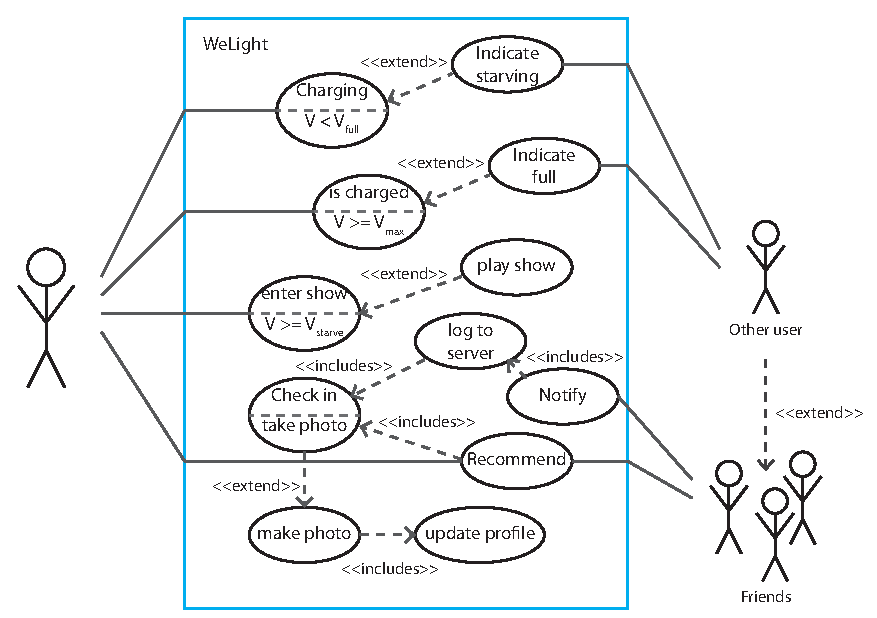
\includegraphics[width=0.8\textwidth]{usecase.pdf}
\caption{UML: Use case diagram of the system}
\label{fig:usecase}
\end{figure}

The sequence diagrams display the different use cases. Figure \ref{fig:sequenceshow} displays regular use of the system in its original design. A show object can detect user IDs by means of RFID tags and then send the instructions via RF signals to the wristbands. These will update their state and loop as long as the battery has a higher energy level than $V_{full}$ as determined in Section \ref{sec:charging}.
%
%------------------- Sequence image
\begin{figure}[h!]
\centering
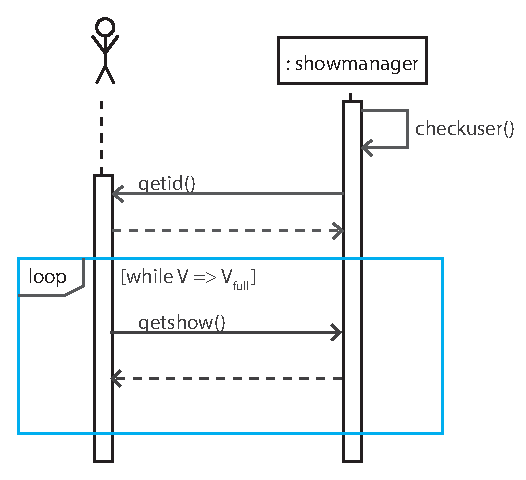
\includegraphics[width=0.5\textwidth]{sequenceshow.pdf}
\caption{UML: Sequence diagram of the regular use of the product}
\label{fig:sequenceshow}
\end{figure}

Figure \ref{fig:sequencecharge} follows this sequence and is initiated whenever the energy level of the battery falls below $V_{full}$. It will indicate towards the environment and other users that the battery is starving. The user can then ask another user for energy or visit an energy bar untill $V_{full}$ is exceeded again. When $V_{max}$ is reached the indication light will turn green as further charging will have no effect. These states are further discussed in Section \ref{sec:states}.
%
%-------------------Sequence image
\begin{figure}[h!]
\centering
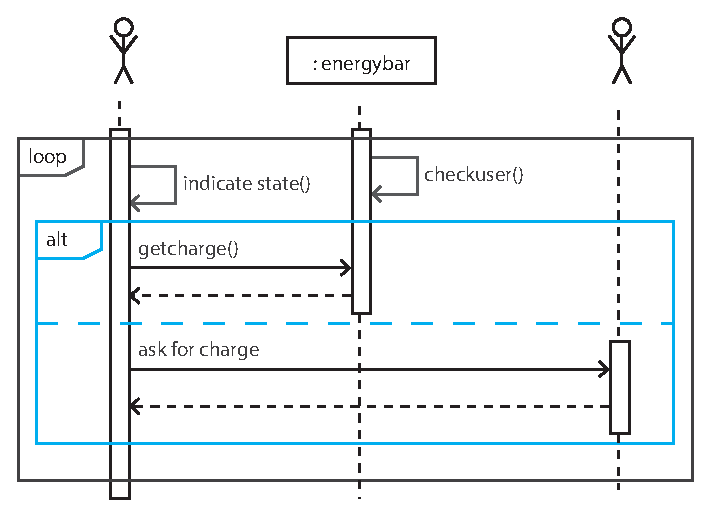
\includegraphics[width=0.7\textwidth]{sequencecharge.pdf}
\caption{UML: Sequence diagram of the charging the system}
\label{fig:sequencecharge}
\end{figure}

Figure \ref{fig:sequenceinternet} shows the sequence diagram whenever a user connects to a checkpoint at the festival. Information about the time of the log, the position of the checkpoint and thus the concurrent nearest festival podium and the user ID is collected and send to the server. The database compares the information with the users personal profile online and the current festival schedule and returns a recommendation. The user can select to inform his/her friends available on the personal profile. They might even add a personal message in order to agree on a meetingpoint. 
%------------------- Sequence diagram image
\begin{figure}[h!]
\centering
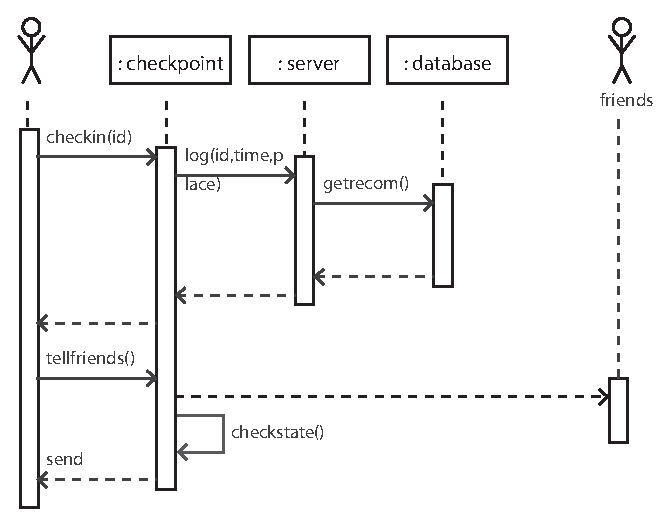
\includegraphics[width=0.7\textwidth]{sequenceinternet.pdf}
\caption{Sequence diagram of the internet of things}
\label{fig:sequenceinternet}
\end{figure}
